\begin{figure}
    \centering
    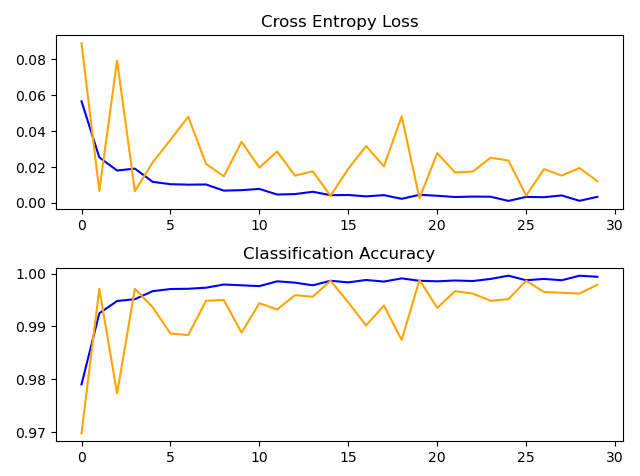
\includegraphics[width = 10cm]{images/squeezenet_30ep_10bat_lfw_full.png}
    \caption{Summary of training a Squeezenet-type Neural Network with 30 epochs of training, a batch size of 20 samples and LFW as a training dataset. The yellow curves represent the actual values, the blue ones are median values. The plot represents a full-size Keras model and uses full \textit{float-32} weights.}
    \label{fig:squeezenet_30ep_10bat_lfw_full}
\end{figure}

\begin{figure}
    \centering
    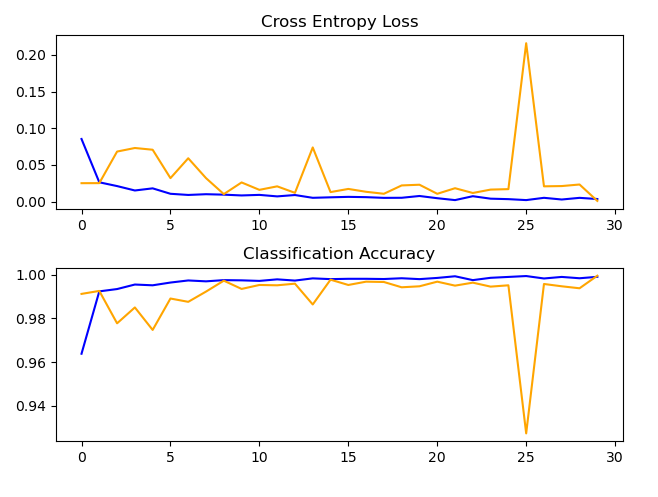
\includegraphics[width = 10cm]{images/squeezenet_30ep_10bat_lfw_tfl.png}
    \caption{Summary of training a Squeezenet-type Neural Network with 30 epochs of training, a batch size of 20 samples and LFW as a training dataset. The yellow curves represent the actual values, the blue ones are median values. The plot represents a quantized Keras model and uses uses \textit{uint8} weights, as any TF-Lite model should. We can see that the TF-Lite model has some pronounced spikes in both accuracy and loss around epoch 20, which might have been caused by the limited representation power of unsinged 8 bit integers.}
    \label{fig:squeezenet_30ep_10bat_lfw_tfl}
\end{figure}